\documentclass[conference]{IEEEtran}
\usepackage{cite}
\usepackage{amsmath,amssymb,amsfonts}
\usepackage{algorithmic}
\usepackage{graphicx}
\usepackage{textcomp}
\usepackage{xcolor}

% our packages
\usepackage{todonotes}
\usepackage[caption=false]{subfig}
\usepackage{url}
\usepackage{enumitem}
\usepackage{listings}
\usepackage{boxedminipage}
\usepackage{comment}
\usepackage{multirow}
\usepackage{xspace}
\usepackage{microtype}
\usepackage[normalem]{ulem}
\usepackage{hyperref}

% our defs
\setlist{noitemsep,leftmargin=*}
\newcommand{\mycomment}[1]{\emph{\textcolor{red}{[#1]}}}

\newcommand{\flushInst}{\texttt{purge}\xspace}
    
\begin{document}

\title{Composable Building Blocks to Open up Processor Design}

\author{\IEEEauthorblockN{Sizhuo Zhang, Andrew Wright, Thomas Bourgeat, Arvind}
\IEEEauthorblockA{MIT CSAIL\\
\{szzhang, acwright, bthom, arvind\}@csail.mit.edu}}

\maketitle

\thispagestyle{plain}
\pagestyle{plain}

\begin{abstract}
    We present a framework called Composable Modular Design (CMD) to facilitate the design of out-of-order processors. In CMD, (1) The interface methods of modules provide instantaneous access and perform atomic updates to the state elements inside the module; (2) Every interface method is guarded, i.e., it cannot be applied unless it is ready; and (3) Modules are composed by atomic rules which call interface methods of different modules. A rule either successfully updates the state of all the called modules or does nothing.
    
    The atomicity properties of interfaces in CMD ensure composability when modules are refined selectively. We show the efficacy of CMD by building an out-of-order RISC-V processor which boots Linux. Modules designed using CMD (e.g., ROB, load-store unit, etc.) can be used and refined by other implementations. We believe that this framework can revolutionize architectural research and practice as the library of reusable components grows.
\end{abstract}

\begin{IEEEkeywords}
    open-source processor, modular design, RISC-V
\end{IEEEkeywords}

\section{Introduction}\label{sec:intro}
It is generally believed that modern processors are the most sophisticated hardware systems that currently exist.
Given the complexity of the design of a processor, it is split into multiple modules, which are often designed by different teams.
This partitioning of work leads to the following two challenges:
\begin{enumerate}
    \item Will the processor work as expected when the modules are composed together?
    \item Is it possible to do \emph{modular refinement}, i.e., refine a module without knowing the implementation details of the other modules?
\end{enumerate}
Ability to do modular refinement is necessary to meet the goal of performance/power/area (PPA), and in some sense it subsumes the functionality challenge. 

Most processors~\cite{rocketchip,boom,fabscalar,pulp} have been designed in a \emph{structural} way, i.e., modules are physical blocks connected by wires.
The implementation of one module may make implicit assumptions about the timing of input signals coming from other modules, and thus, the composed processor functions correctly if each module meets its timing assumptions and functionality.
Such timing assumptions are difficult to specify, which makes the mechanical verification of timing-assumption violations impossible.
In order to avoid rigid timing assumptions, some designers use the latency-insensitive framework, where modules communicate with each other using FIFOs.
In such frameworks, a module cannot depend on the timing of other modules, and that significantly improves the flexibility in modular refinement.
Although the latency-insensitive framework has proven useful in building hardware accelerators, it is not expressive enough for processors. 
In processors, a microarchitectural event may need to access and modify the states in multiple modules \emph{atomically}. 
This is because different microarchitectural events may race with each other in accessing the states inside modules, and such ``data races'' can make the processor implementation incorrect if an event fails to perform all its accesses atomically with respect to other events.
Here we list several race cases in the out-of-order (OOO) processor we have built, and we will discuss a detailed example later in Section~\ref{sec:cmd:iq}:
\begin{enumerate}
    \item \emph{Speculation bits}:
    Often an instruction flowing through the execution pipeline carries bits to indicate the speculation events which can cause its squashing.
    There is a race in the management of these bits, because they are cleared by asynchronous events that show that the speculations were correct.
    
    \item \emph{Memory address disambiguation}:
    A load in the load queue searches the store queue for forwarding.
    At the same time, a store in the store queue may get its address filled, and it searches the load queue for detecting memory-dependency violations. 
    There is a race if the addresses are the same.
    
    \item \emph{Partially overlapped addresses}:
    We stall the execution of a younger load-word if there is an older store-byte on the same word.
    For example, a load-word searches older stores for detecting such stalls. % due to partially overlapped addresses,
    A store-byte should wake up younger loads stalled by it when the store is written to the L1 cache.
    There is a race if the load and store are accessing the same word.
    
    \item \emph{Distributed cache coherence protocols}:
    A race condition arises when a parent is trying to downgrade a child's entry while it is receiving the eviction of the same entry from the child.
\end{enumerate}

A non-modular solution to these race problems is to put all the interacting components in one module.
However, doing so in complex designs leads to big monolithic modules.

In this paper, we present the \emph{Composable Modular Design (CMD)} framework, which permits state changes in multiple modules \emph{atomically}.
CMD uses the following two techniques to achieve composability and atomicity:
\begin{enumerate}
    \item \emph{modules with guarded interface methods}, and
    \item \emph{atomic rules} that glue modules together by calling the methods of modules.
\end{enumerate}

In CMD, a module is like an object in an object-oriented programming language, and can be manipulated only by its interface methods.
A method provides combinational access and performs atomic updates to the state elements inside the module.
In addition, every interface method is \emph{guarded}, that is, there is an implicit guard (a ready signal) on every method which must be true before the method can be invoked (enabled).
For example, the guard signal for the enqueue method of a FIFO is simply the not-full condition.
CMD subsumes the traditional latency-insensitive framework by admitting systems where each interface method of every module simply enqueues or dequeues FIFOs.

Unlike the structural designs, modules in CMD are manipulated by the special glue logic, i.e., atomic rules, which is a collection of calls to the methods of one or more modules.
An atomic rule is like an atomic transaction, which either updates the states of all the called modules  or does nothing.
Of course, a method can execute only if its guard is true; therefore, the guards of all the methods called by a rule must be true simultaneously.
In CMD, each microarchitectural event, which is supposed to happen in a single cycle, is expressed as an atomic rule.
Atomicity ensures that the refinement of a module does not affect how the module is used by other rules.

This paper makes the following contributions:
\begin{enumerate}
    \item Composable Modular Design (CMD) flow, a new framework for implementing complex and realistic microarchitectures;
    
    \item A parameterized and modular OOO processor, \emph{RiscyOO}, built using the CMD framework, which is released at \texttt{\url{https://github.com/csail-csg/riscy-OOO}} under the MIT License;
    
    \item Applications of the CMD framework and the RiscyOO processor.
\end{enumerate}

\noindent\textbf{Paper organization:}
Section~\ref{sec:related} presents related works.
Section~\ref{sec:cmd} describes the CMD framework.
Section~\ref{sec:ooo} introduces the RiscyOO processor built using CMD.
Section~\ref{sec:app} discusses further applications of CMD and RiscyOO.
Section~\ref{sec:conclude} concludes the paper.

\section{Related Work}\label{sec:related}
There is a long history of processors that were designed in the academic setting.
Many of these attempts were focused on demonstrating new architectures; there was no expectation that other people would refine these implementations.
Other attempts aimed at providing open-source processors and corresponding frameworks for configuring the designs.
For example, the Rocket chip generator~\cite{rocketchip} can generate SoCs with RISC-V cores that are parameterized by caches, branch predictors, ISA extensions, etc.
Fabscalar~\cite{fabscalar} allows one to assemble different superscalar designs from a set of predefined pipeline-stage blocks.
FabScalar has been successful in generating heterogeneous cores, but the predefined blocks are not intended to be modified.
PULP~\cite{pulp} is a platform for designing low-power SoCs, but the processor cores are not intended to be refined within the framework.

All these frameworks are structural compositions of predefined building blocks.
The goal of our CMD framework is more ambitious, in the sense that, in addition to parameterized designs, we want the users to be able to incorporate new microarchitectural ideas.
For example, replace a centralized instruction-issue queue with several instruction-issue queues, one for each functional unit.
Traditionally, making such changes requires a deep knowledge of the internal functioning of the other blocks, otherwise, the processor is unlikely to function. 
We want to encapsulate enough properties in the interface of each block so that it can be composed without understanding the internal details.

\section{Composable Modular Design (CMD) Framework}\label{sec:cmd}

As mentioned in Section~\ref{sec:intro}, latency-insensitive frameworks are insufficient for processor designs because of races between microarchitectural events.
We first study an example race case which involves the instruction-issue queue (IQ) in the OOO processor, and then show how CMD maintains atomicity and solves the race problem by extending module interfaces with concurrency properties.

\subsection{Race between Microarchitectural Events}\label{sec:cmd:iq}
Figure~\ref{fig:race:modules} shows the modules and microarchitectural events that participate in a race in the OOO processor.
Module IQ keeps unissued instructions and tracks whether their (physical) source registers are ready or not.
Module RDYB keeps one bit for each physical register, indicating whether the register has valid data or not.
Microarchitectural event {Rename} gets a new instruction from the decode stage, does renaming, \emph{checks} RDYB to see if the source registers of the instructions are ready, and \emph{enters} the instruction with the register-ready bits into IQ.
Microarchitectural event {RegWrite} happens at the end of execution pipeline when an instruction gets the value for its destination register.
The event \emph{sets} the corresponding bit in RDYB and \emph{wakes} up dependent instructions in IQ.
(There are other actions performed by the two events, but they are unrelated to the race case.)

Both events are accessing the states in IQ and RDYB, thus forming a race.
If Rename does not happen atomically with respect to RegWrite, then the race can lead to deadlock in the processor.
Consider the case in Figure~\ref{fig:race:deadlock}.
Rename is processing instruction $I$ with physical source register $P3$, while RegWrite is writing the same register $P3$.
It is possible that Rename first checks RDYB and finds $P3$ not ready, then RegWrite happens and cannot wake up instruction $I$ which is not yet in IQ, and finally Rename enters $I$ into IQ.
In this case, $I$ will be stuck in IQ forever, i.e., the processor deadlocks.

It is difficult for latency-insensitive frameworks to keep the atomicity of events and resolve this race problem.
A structural solution is to introduce bypass wires either in RDYB (to have Rename see the updated register-ready bits) or in IQ (to have RegWrite wake up instruction $I$).
However, the bypass wires break latency insensitivity and reduce composability.

\begin{figure}[!htb]
    \centering
    \subfloat[Modules and microarchitectural events involved in the race. Modules IQ and RDYB are represented by blocks, while microarchitectural events Rename and RegWrite are represented by clouds. Event Rename calls method \emph{check} of RDYB and method \emph{enter} of IQ. Event RegWrite calls method \emph{set} of RDYB and method \emph{wake} of IQ.\label{fig:race:modules}]{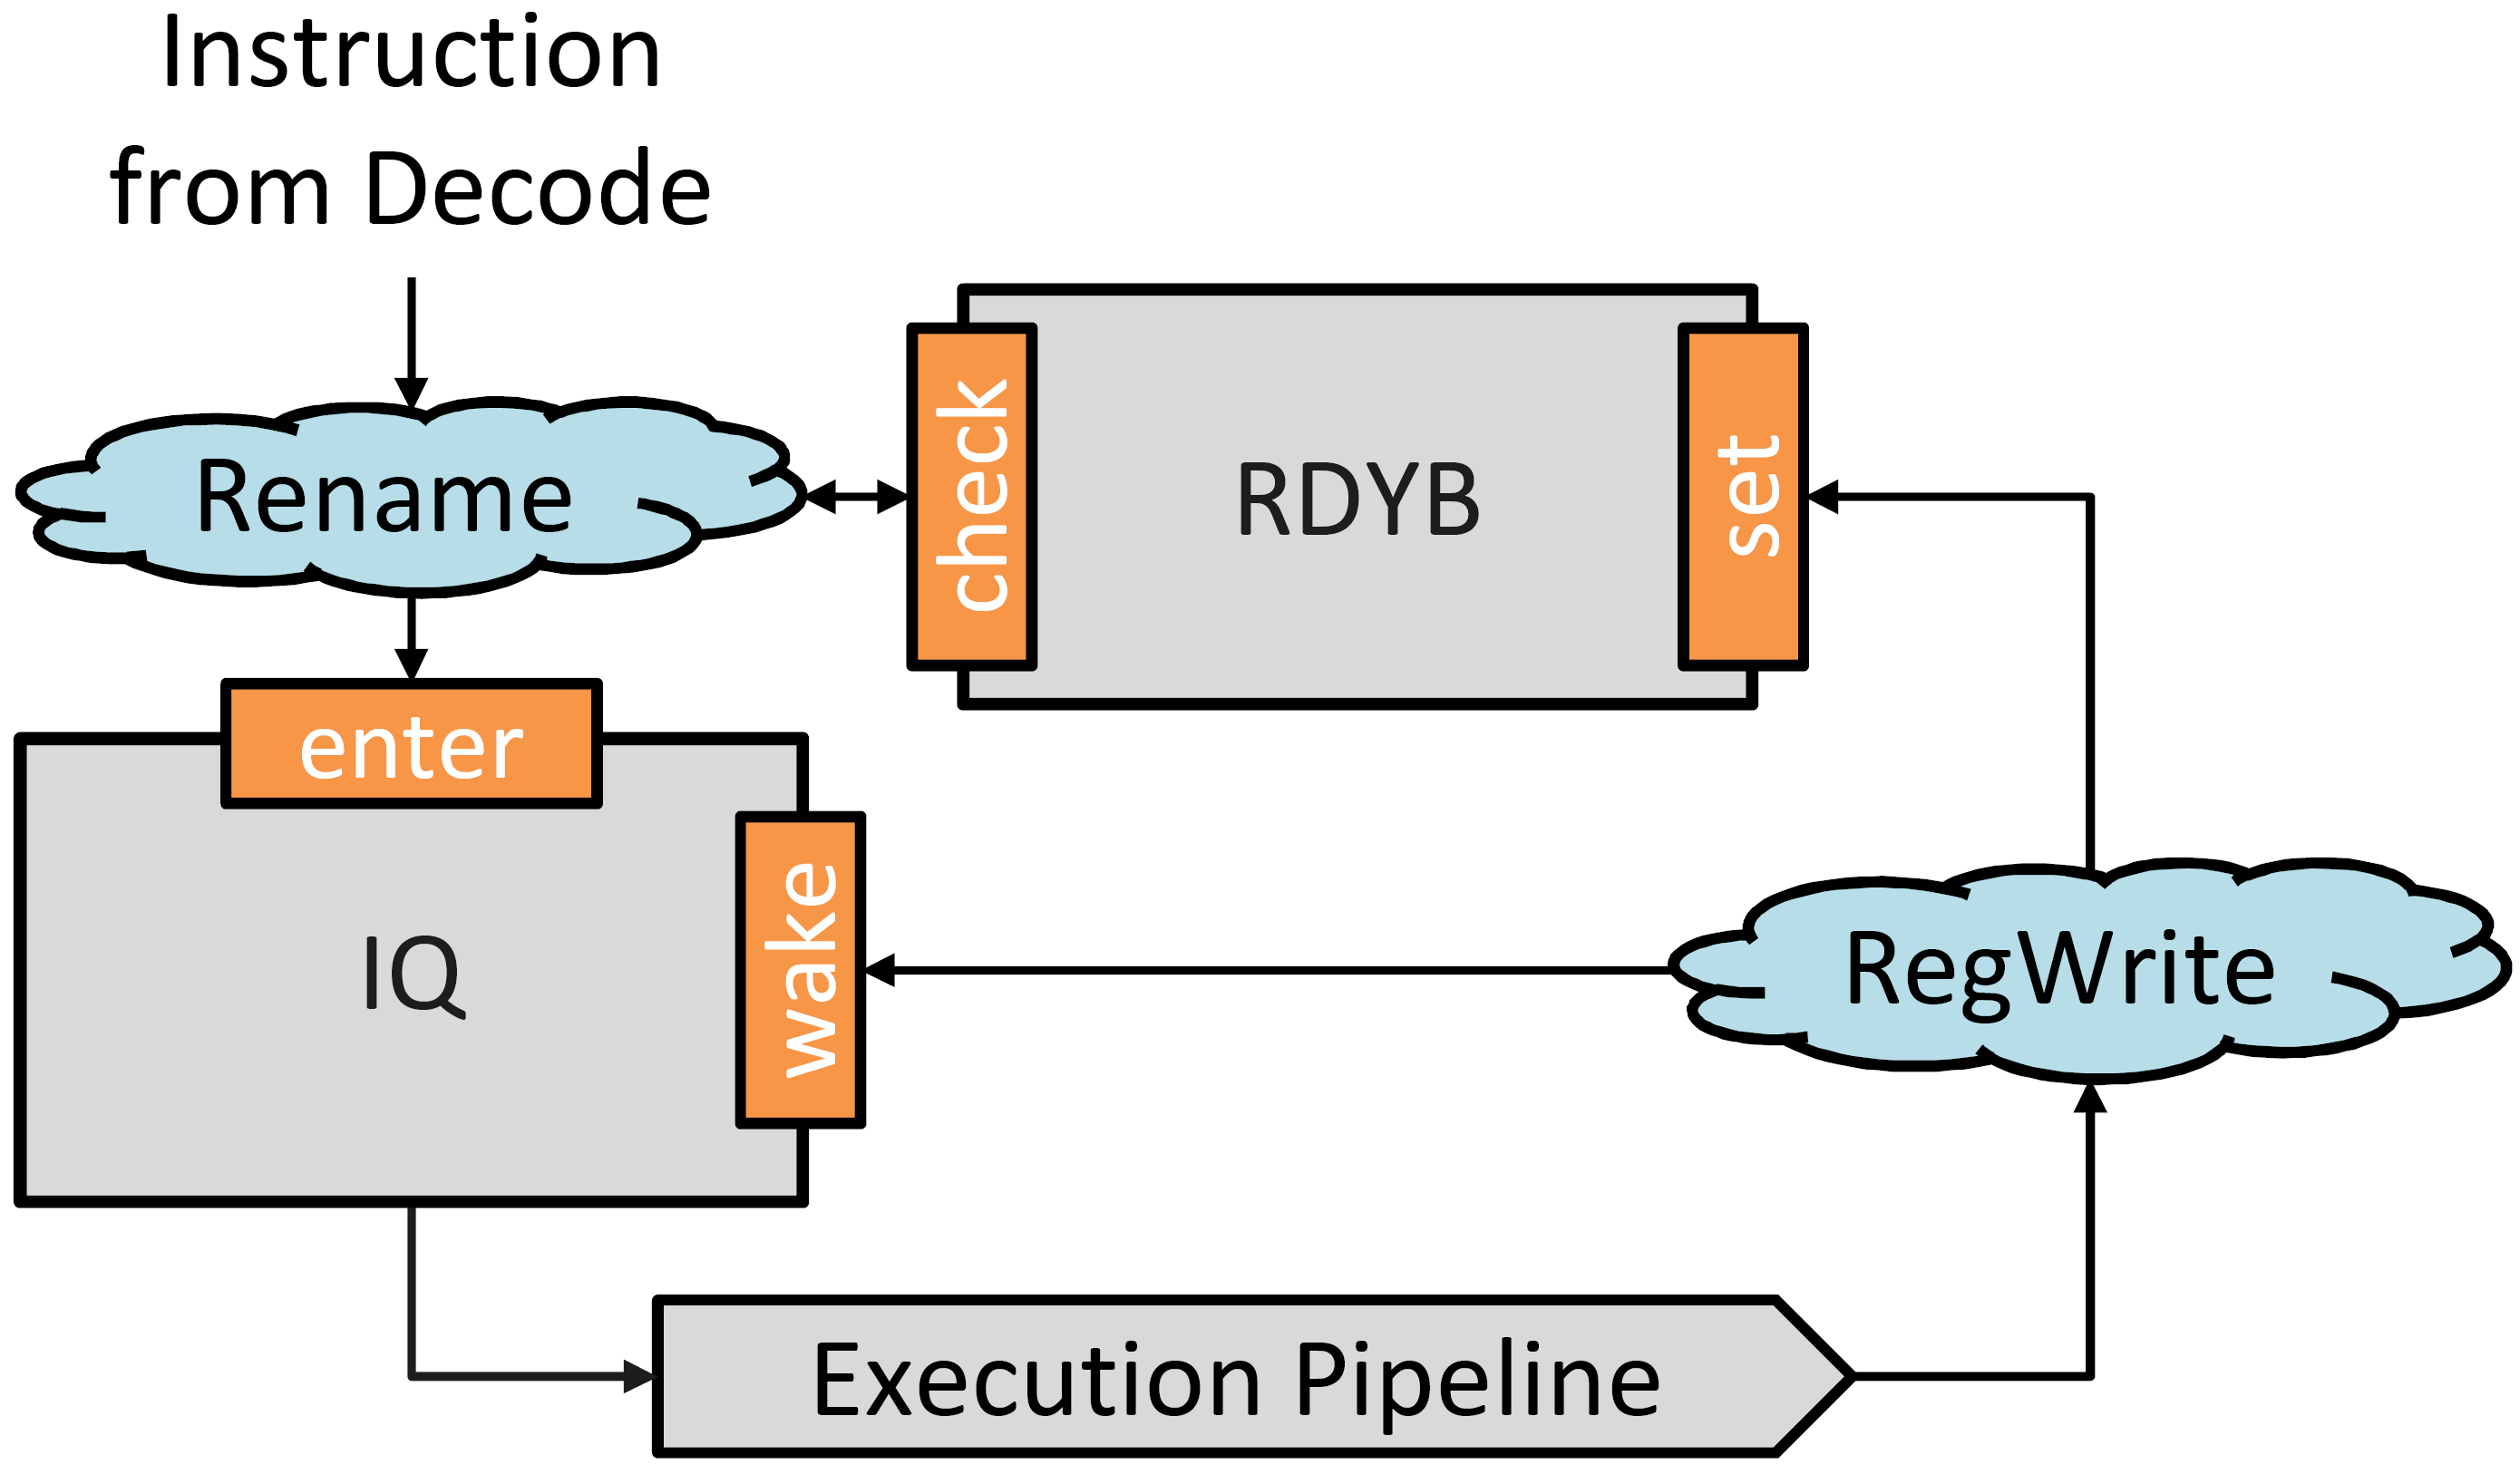
\includegraphics[width=0.8\columnwidth]{race.PNG}}\\
    \subfloat[Operation sequence that leads to deadlock. Event Rename is processing instruction $I$ with source register P3 while event RegWrite is writing P3.\label{fig:race:deadlock}]{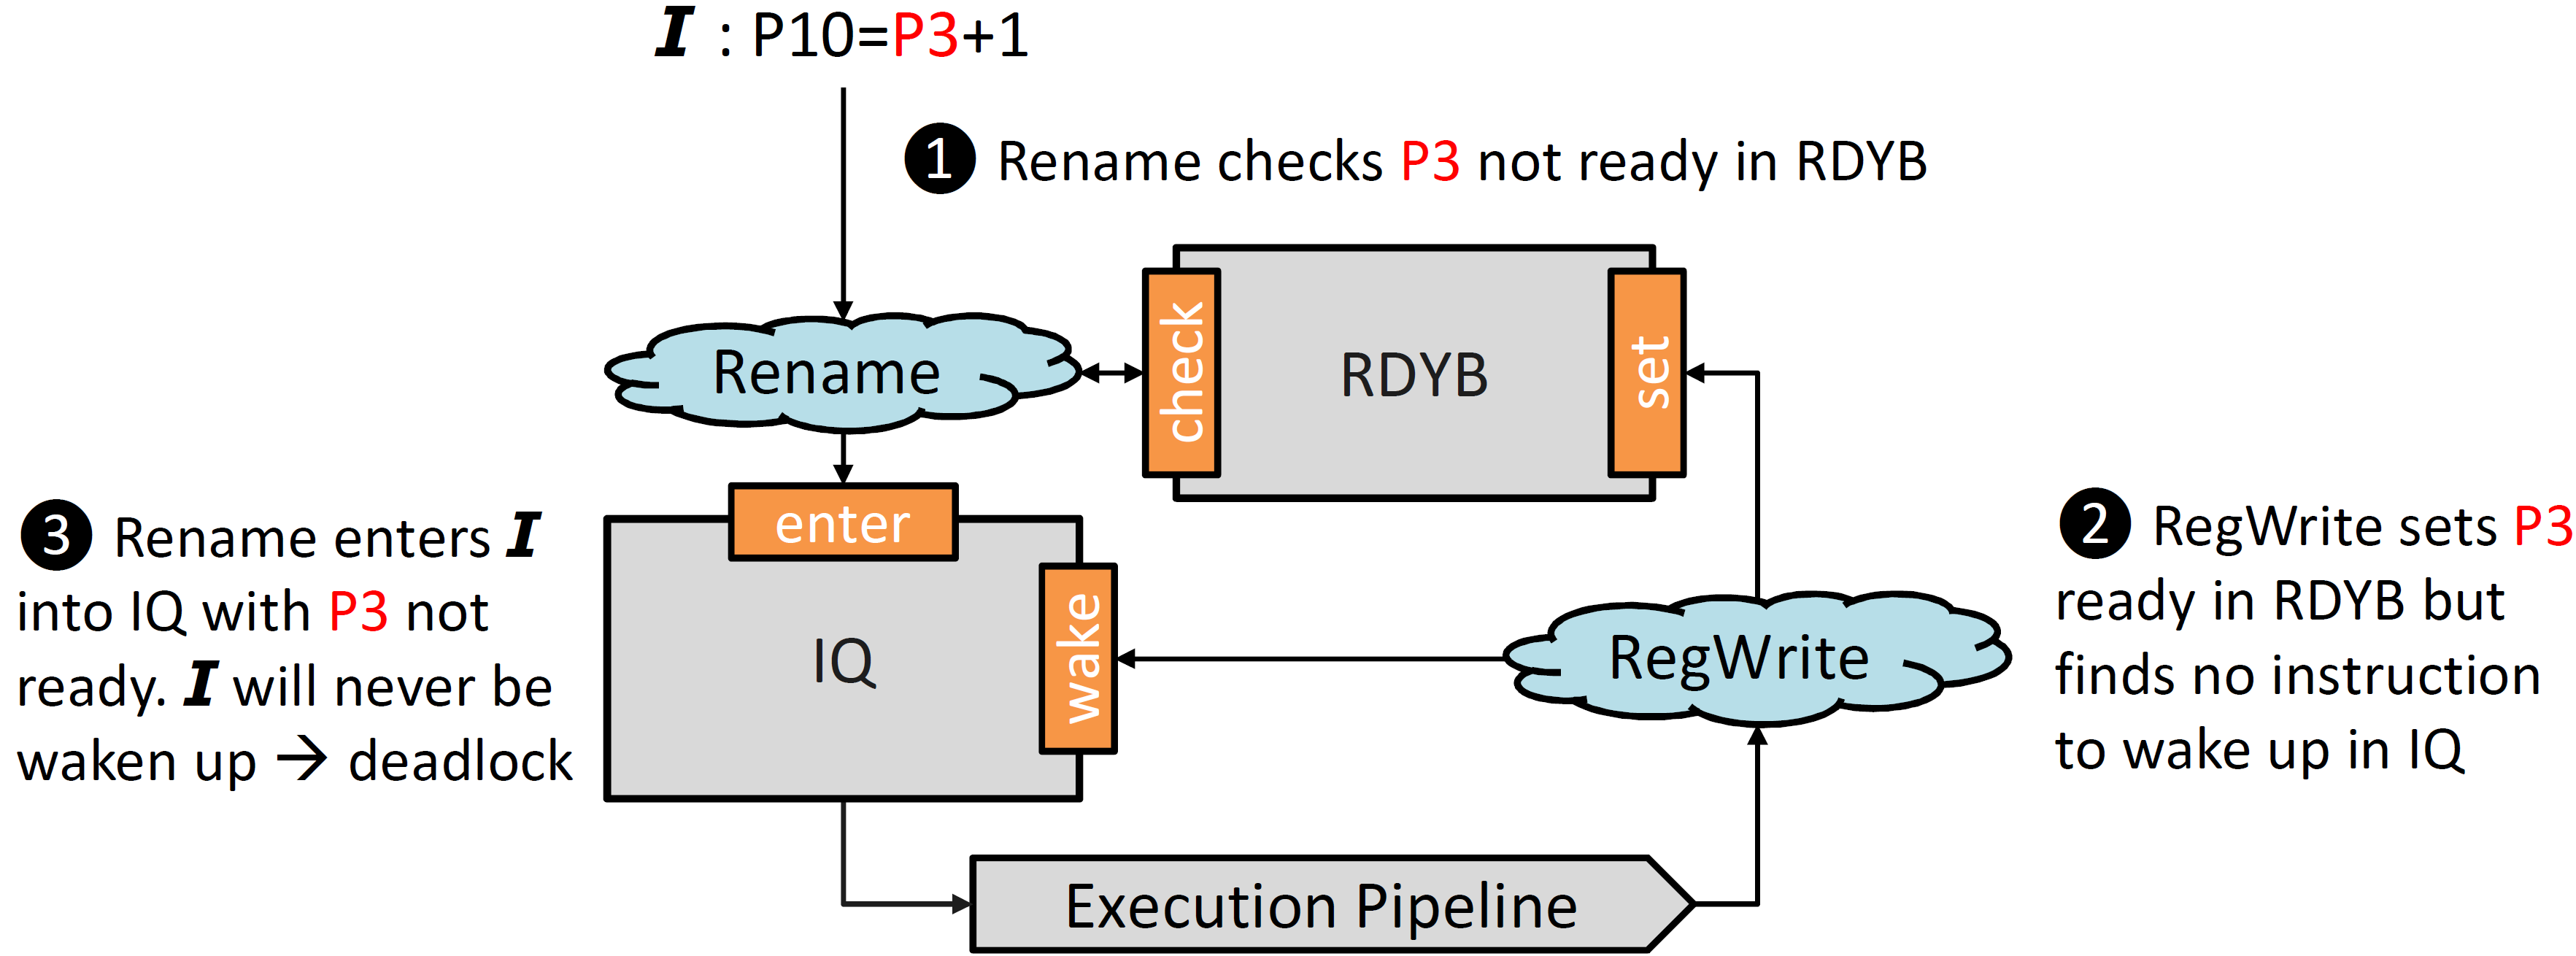
\includegraphics[width=\columnwidth]{deadlock.PNG}}
    \caption{Race between microarchitectural events Rename and RegWrite in an OOO processor}\label{fig:race}
\end{figure}

\subsection{Maintaining Atomicity in CMD}
To resolve the race problem in Figure~\ref{fig:race}, CMD expresses events Rename and RegWrite as two separate rules and guarantees the atomicity of each rule.
That is, event Rename will be expressed as rule Rename which calls method \emph{check} of RDYB and method \emph{enter} of IQ, and event RegWrite will be expressed as rule RegWrite which calls method \emph{set} of RDYB and method \emph{wake} of IQ.
However, enforcing atomicity is challenging because the two rules manipulate the same states.
In this case, it has to be ensured that the rules appear to execute one after another.
Whether two rules can execute concurrently and in which order depend on the properties of the called methods.
Thus, for each module, we use a \emph{Conflict Matrix (CM)}, which specifies which methods of the module can be called concurrently.
The relation between each pair of methods may be described as follows:
\begin{itemize}
    \item \emph{conflict-free}: the methods do not manipulate the same states, and thus, can be called concurrently;
    \item \emph{conflicting}: the methods cannot be called in the same cycle;
    \item \emph{happen-before}: the methods can be called concurrently but functionally they behave as if one executed before the other.
    This involves bypass logic inside the module in case a write method happens before a read method.
\end{itemize}
Given the CMs of all the modules, it is straightforward to derive the concurrency relation between every pair of rules.
Support for CMD requires a stall signal in the glue logic to suppress the execution of one rule in a pair of conflicting rules.

Back to the race problem in Figure~\ref{fig:race}, if there is no bypass wire in the implementation of module IQ or module RDYB, then the CM of IQ will have method \emph{wake} happen before \emph{enter}, and the CM of RDYB will have method \emph{check} happen before \emph{set}.
In this case, rules Rename and RegWrite conflict with each other and must be executed one by one. CMD will generate a stall signal to enforce such a schedule.
To make rules RegWrite and Rename execute concurrently, one solution is to change the CM of RDYB to have method \emph{set} happen before \emph{check}.
That is, the implementation of RDYB contains a bypass wire from method \emph{set} to \emph{check}.
We will show shortly that this bypass wire can be generated implicitly in CMD.
In this case, RegWrite will appear to execute before Rename.

\subsection{Expressing CMD in Hardware Description Languages (HDLs)}
We expressed the CMD framework in Bluespec System Verilog (BSV).
The BSV compiler automatically (1) derives the CM for each module implementation, (2) derives the concurrency relations between each pair of rules according to the CMs, and (3) generates stall signals in the glue logic.
\emph{The compiler statically resolves all the dynamic concurrency issues, making it possible to apply mechanical verification  techniques to designs.}

It is possible to use other HDLs to express CMD, but then we may not get all the benefits of the automatic concurrency analysis done by the BSV compiler.

\subsection{CMD Design Flow}
We develop designs in two phases.
We first focus on functionality and do not try to get maximum hardware concurrency.
After this phase, we often discover that two rules are conflicting, and this affects performance adversely.
To execute such rules concurrently invariably requires introduction of bypass logic.
In CMD, one never writes bypass logic explicitly.
Instead, one can specify the order in which rules should execute, from which one can derive the desired CM of each module.
Rosenband and Arvind~\cite{rosenband2005hardware} have given a systematic way to transform the module implementation to satisfy a given CM using Ephemeral History Registers (EHRs) which implicitly introduce bypass logic.
This transformation does not affect the functional correctness of the overall design.

\subsection{Modular Refinement in CMD}
When a refinement on a module does not affect the interface methods or the CM, the local correctness of the module guarantees the preservation of the overall correctness.
If the CM of the refined module is changed, the BSV compiler can re-analyze the relations between rules and generate new stall signals to keep the design functionally correct.

In some cases, a refinement may entail several modules simultaneously or may add new methods to a module for increased functionality.
Any changes in interface methods imply that the rules that call these methods have to be changed.
However, making this change does not require knowing the internal details of other modules, because other modules have been encapsulated by their interface specifications.

In summary, by employing modules with guarded interfaces and atomic rules, CMD is able to provide strong composability and atomicity.


\section{RiscyOO -- a RISC-V Out-of-Order Processor Designed Using CMD}\label{sec:ooo}
Using the CMD framework, we built \emph{RiscyOO}, a parameterized out-of-order superscalar cache-coherent multiprocessor.
The processor uses the open-source RISC-V instruction set~\cite{riscv}.
Figure~\ref{fig:ooo} shows the structure of RiscyOO multiprocessor.
The OOO core contains 2-way superscalar fetch/decode/commit, 4 execution pipelines, and two-level private TLBs.
The core also performs various branch predictions, and execute loads speculatively.
Figure~\ref{fig:tlb-config} shows one possible configuration of a single core.
Multiple cores can be connected to a non-blocking coherent cache hierarchy to form a multiprocessor.

\begin{figure}[!htb]
    \centering
    \subfloat[Top-level moduels and rules of the OOO core. Modules are represented by rectangles, while rules are represented  by clouds. The core contains four execution pipelines: two for ALU and branch instructions, one for memory instructions, and one for floating point and complex integer instructions (e.g. multiplication). Only two pipelines are shown here for simplicity.\label{fig:ooo:core}]{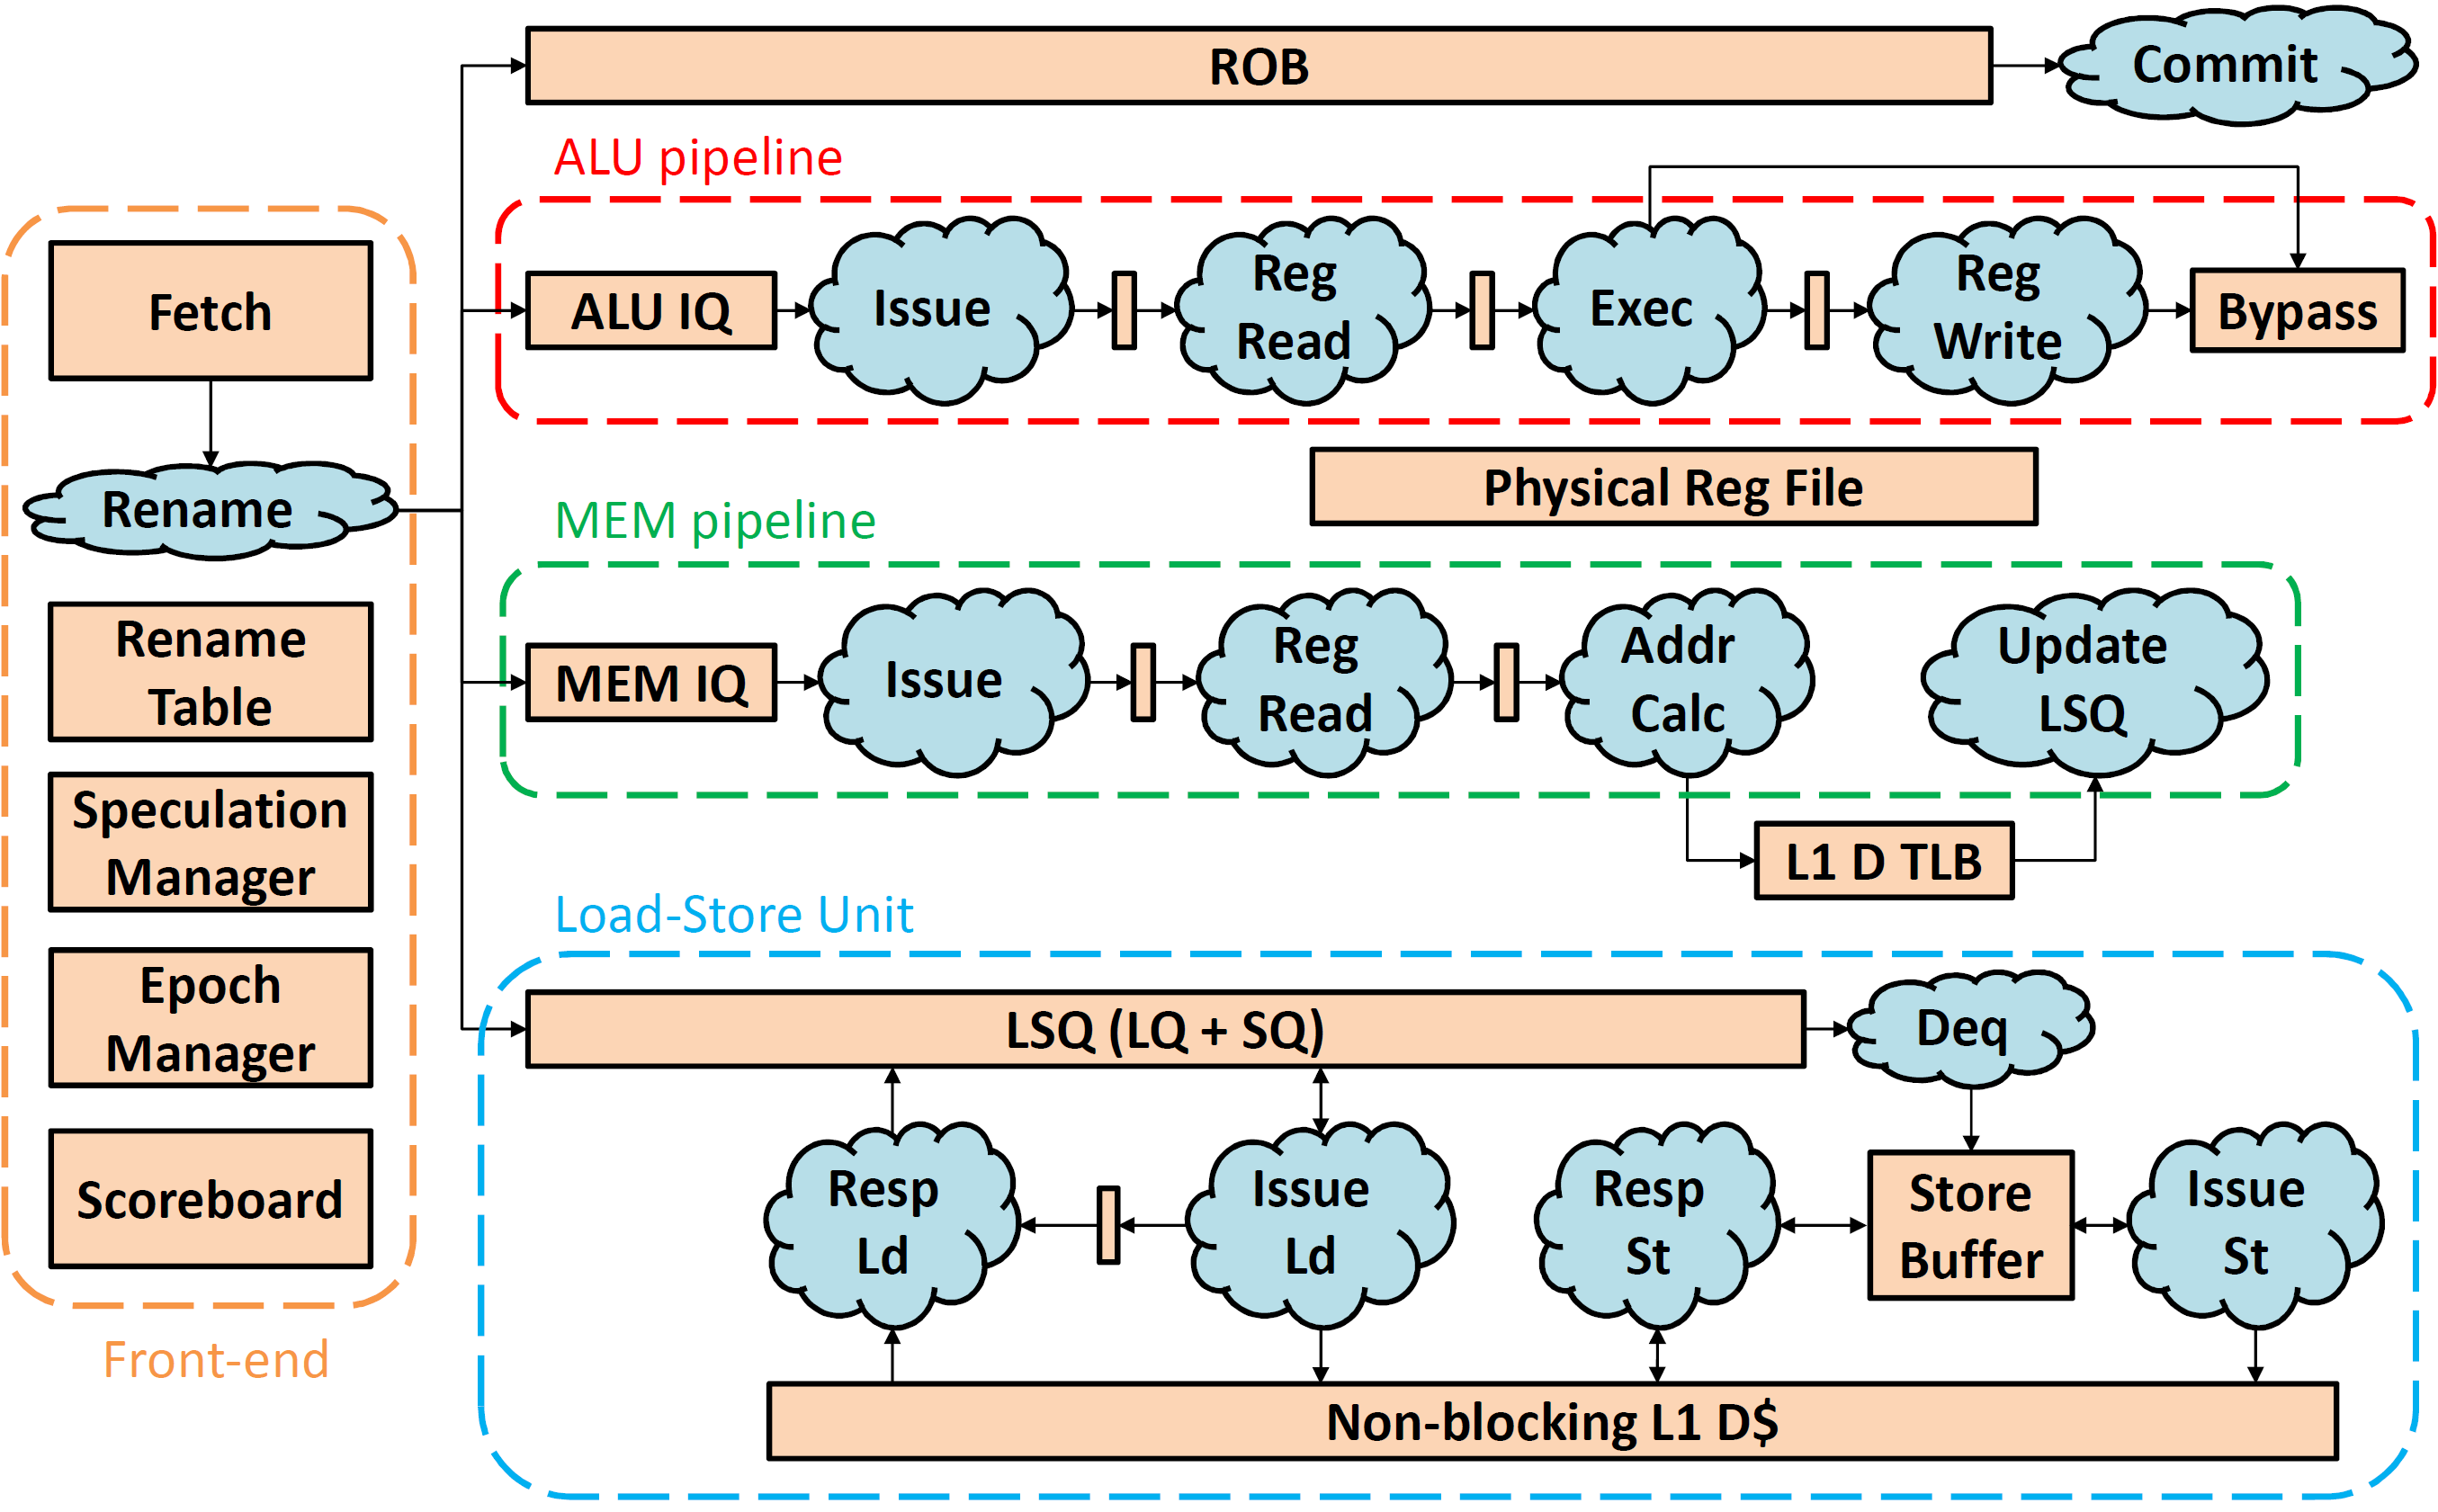
\includegraphics[width=\columnwidth]{core.PNG}}\\
    \subfloat[Connecting OOO cores to form a multiprocessor\label{fig:ooo:mem}]{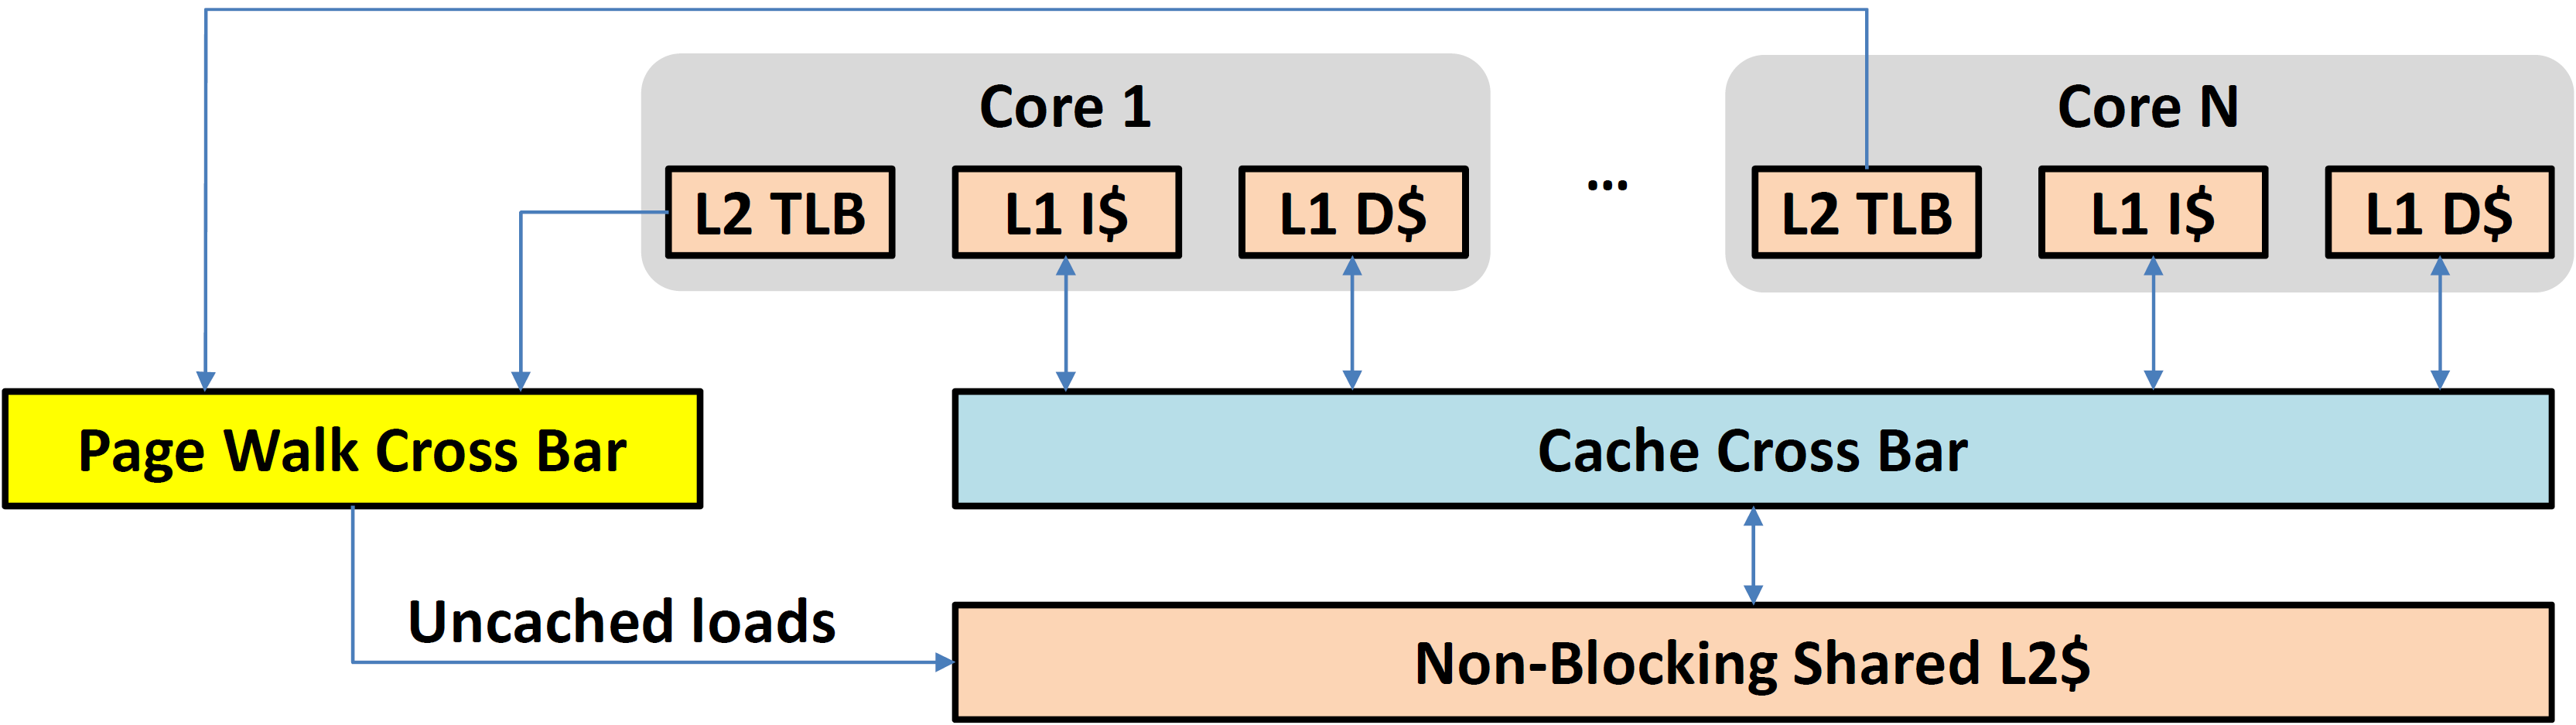
\includegraphics[width=0.9\columnwidth]{mem.PNG}}
    \caption{RiscyOO multiprocessor}\label{fig:ooo}
\end{figure}

We prototyped RiscyOO on AWS F1 FPGA~\cite{awsf1}, and booted Linux on it.
To evaluate the performance of RiscyOO, we run SPEC CINT2006 benchmarks (ref input size, no sampling) which ran trillions of instructions on our FPGA prototype without any hardware failures.
Our evaluation shows that RiscyOO is much faster than in-order processors, and matches state-of-the-art academic out-of-order processors.
However, commercial ARM-based processors are 40\% faster than RiscyOO on average in terms of cycle counts, possibly because of the higher superscalarity and more sophisticated microarchitectures.
Detailed performance analysis can be found in \cite{riscyoo}.

We also applied standard ASIC synthesis flow (topographical synthesis) on RiscyOO.
Using a 32nm technology, the processor can be clocked over 1GHz.


\section{Applications of CMD and RiscyOO}\label{sec:app}

\subsection{Flexible Open-Source Processor IP}
The software community has benefited for years from open-source projects and permissive licensing. 
This has allowed reusable libraries with proper APIs to flourish. 
The open-source RISC-V ISA~\cite{riscv} is an attempt to open up the processor-design community in a similar way.
Although there are already several good and free implementations of RISC-V processors~\cite{rocketchip,boom,pulp}, which can be included directly as processor IP blocks when building SoCs, they are not enough to realize the full potential of RISC-V.
This is because these processors are built in a structural way.
As a consequence, their customizability is at a coarse granularity (e.g., changing cache and buffer sizes) and often limited by the number of configurations provided by the original processor designers.
Moreover, if one needs to change the implementations of one or more modules in the processor, then he/she may need to understand the implementations of nearly all the modules in order to prevent his/her changes from breaking the whole processor.
This requires significant effort, which may be comparable to building a new processor from scratch, and we think it would intimidate people from reusing or customizing these processor IPs.

The CMD framework solves the problem by providing composability at the module level, and thus enables customization at a much finer granularity.
If people need to change a module in a processor designed using CMD, only the interfaces, instead of implementations, of other modules need to be understood.
This lowers the barrier for customizing processor designs, and would encourage more people to join the open-source hardware community.
Furthermore, CMD allows people to contribute a variety of modules and replacements, which can be composed easily using atomic rules to form processors suitable for different use cases.
As an example, we discuss next two of the refinements of RiscyOO that we have implemented. 

\noindent\textbf{Refining the TLB microarchitectures:}
In the original design of RiscyOO, both L1 and L2 TLBs block on misses, and an L1-D TLB miss blocks the memory execution pipeline.
To improve performance, we have changed the L1-D TLB and L2 TLB to support parallel miss handling and to allow hits-under-misses.
To reduce the TLB miss latency, we also included in the L2 TLB a ``split translation cache''~\cite{translationCache}, which caches intermediate page-walk results.
These refinements not only change the internal implementations of TLBs significantly, but also affect the interfaces of TLBs, e.g., the L1-D TLB sends responses out of order.
Thanks to CMD, the changes in TLBs affect only rules that call the TLB interface methods (e.g., rules AddrCalc and UpdateLSQ in Figure~\ref{fig:ooo:core}). One person was able to make these  changes within two weeks.
We evaluated the performance impact of these refinements using SPEC CINT2006 benchmarks~\cite{riscyoo}.
Figure~\ref{fig:tlb-config} shows the configuration of the baseline processor which has blocking TLBs.
Figure~\ref{fig:tlb-refine} shows the details of the refinements, i.e., the number of parallel misses of TLBs and the size of the translation cache.
Figure~\ref{fig:tlb-data} shows the relative performance improvement caused by the refinements.
The improvement turns out to be significant: the average is 31.6\% (right-most column), and the maximum even reaches 98\% (benchmark astar).

\begin{figure}[!htb]
    \centering
    \subfloat[Base processor configuration\label{fig:tlb-config}]{%
    \footnotesize
    \begin{tabular}{|l|l|}
        \hline
        Front-end & 2-wide superscalar fetch/decode/rename \\
                  & 256-entry direct-mapped BTB \\
                  & tournament branch predictor as in Alpha 21264 \\
                  & 8-entry return address stack \\ \hline
        Execution & 64-entry ROB with 2-way insert/commit \\
        Engine    & Total 4 pipelines: 2 ALU, 1 MEM, 1 FP/MUL/DIV \\
                  & 16-entry IQ per pipeline \\ \hline
        Ld-St Unit& 24-entry LQ, 14-entry SQ, 4-entry SB (each 64B wide) \\ \hline
        TLBs      & Both L1 I and D are 32-entry, fully associative \\
                  & L2 is 2048-entry, 4-way associative \\ \hline
        L1 Caches & Both I and D are 32KB, 8-way associative, max 8 requests \\ \hline
        L2 Cache  & 1MB, 16-way, max 16 requests, coherent with I and D \\ \hline
        Memory    & 120-cycle latency, max 24 req (12.8GB/s for 2GHz clock) \\ \hline
    \end{tabular}%
    }\\
    \subfloat[Summary of TLB refinements\label{fig:tlb-refine}]{%
    \footnotesize
    \begin{tabular}{|p{10ex}|p{50ex}|}
        \hline
        L1 D-TLB & Max 4 misses \\ \hline
        L2 TLB & Max 2 misses, max 2 page walks in parallel \\ \hline
        Translation Cache & 24 fully associative entries for each non-leaf page-walk level. Total 2 non-leaf page-walk levels. \\ \hline
    \end{tabular}%
    }\\
    \subfloat[Performance improvement (in percentage) caused by the TLB refinements\label{fig:tlb-data}]{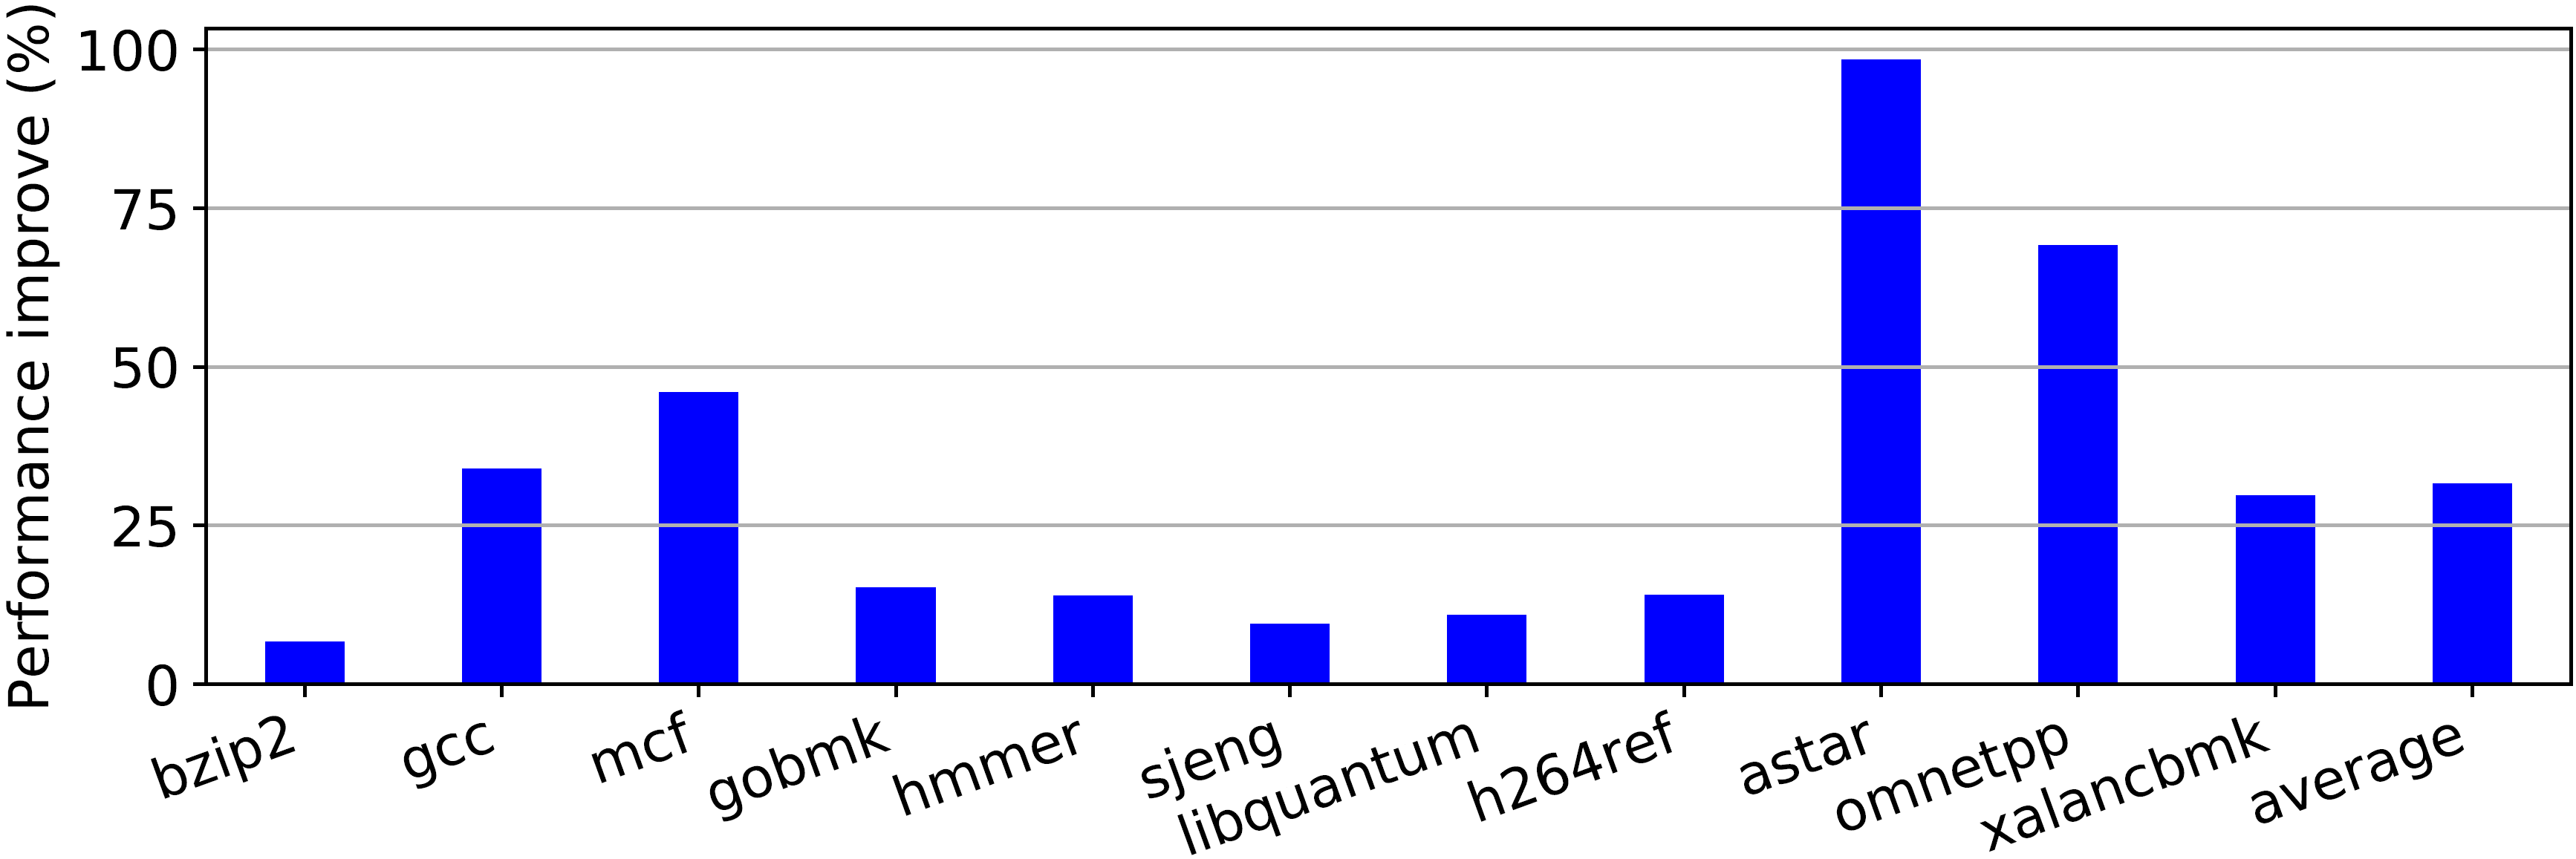
\includegraphics[width=\columnwidth]{spec_tlb_opt_improve.PNG}}
    \caption{Evaluation of TLB refinements\label{fig:tlb}}
\end{figure}

\noindent\textbf{Adding support for TSO:}
The original design of RiscyOO supported only weak memory models, e.g., WMM~\cite{wmm} or GAM~\cite{gam}.
To make RiscyOO support TSO, we have changed the design of the load-store unit and L1-D cache so that cache evictions from L1-D will be snooped by the load-store queue (LSQ in Figure~\ref{fig:ooo:core}).
These changes require adding new interface methods, e.g., a new method in LSQ that kills eagerly executed loads when a cache eviction happens.
This new method can race with other existing methods in LSQ, e.g., the one that issues a load from LSQ.
Thanks to CMD, we can resolve these race conditions easily by relying on conflict matrices and rule-atomicity.
The TSO support was added by one person in two weeks.
We ran PARSEC benchmarks on a 4-core configuration of RiscyOO, and showed that the TSO refinement has little performance impact~\cite{riscyoo}.

To foster the open-source community, we have released our building blocks for the RiscyOO processor at \texttt{\url{https://github.com/csail-csg/riscy-OOO}} under the MIT License.
As the number of refinements on our design provided by us and the community grows over time, we hope these building blocks can become a toolbox for computer architects and SoC designers.

\subsection{Secure Architectures}
The recent advent of side-channel attacks based on speculative microarchitectures have prompted architects to redesign processors for security.
Such redesigns often manipulate microarchitectural states differently, and inevitably require changes in both software and hardware.
RiscyOO is a great platform for exploring security solutions because its speculative microarchitecture is as vulnerable to side-channel attacks as commercial processors.
Its easy-to-modify design allows fast exploration of new security schemes which can be tested while running full software stack.
Since all the reported attacks can be replicated even in an FPGA implementation, a red team can directly try to break a supposedly ``secure'' processor running in the (AWS) cloud.
Last but not the least, the high speed of RiscyOO (40MHz on AWS FPGA) makes it possible to evaluate security schemes using large realistic benchmarks.

We have recently proposed a secure processor architecture based on RiscyOO (citation suppressed for blind reviews).
The realistic microarchitecture of RiscyOO has helped us identify subtle issues in implementing security features, and CMD has enabled us to resolve these problems swiftly.
For example, we implemented a new \flushInst{} instruction, which the software can use to scrub local microarchitectural states while switching context. This blocks side-channels between programs that runs on the core before and after the context switch.
When the \flushInst{} instruction reaches the commit stage, it first stops instruction-fetch and then squashes all the in-flight instructions.
After that, it starts flushing all the stateful modules including TLBs, L1 caches, branch predictors, etc.
Instruction-fetch will be resumed after all the flushes have completed.

Although the implementation of \flushInst{} could reuse the squash mechanism of exception handling, we discovered subtle issues regarding the race between the flush of stateful modules and the activity of wrong-path instructions which are squashed but have not yet been removed from the pipeline.
Figure~\ref{fig:fetch} shows the 4-stage pipeline inside module Fetch.
When a squash happens, the instructions in the FIFOs Q1 and Q2 correspond to the in-flight requests in I-TLB and I-cache, respectively, and should not be removed immediately; otherwise the in-flight requests in the I-TLB and I-cache will become orphans.
Instead of propagating squash signals into module Fetch, rule Rename will drain these wrong-path instructions gradually using an epoch-based scheme.
However, a wrong-path instruction in Q1 can then issue a wrong-path request to I-cache in rule Fetch2, while the I-cache is being flushed.
A straightforward implementation is to block the request interface of I-cache during the flush.
However, this implementation is insecure, because wrong-path instructions may leave their footprints in I-cache after the flush completes, and create a side-channel to influence the program after the context switch.
Our implementation makes use of the guarded interface in CMD.
The guard of the start-flush method of module Fetch can be true only when all the pipeline FIFOs in Fetch are empty.
The guard ensures that flush can be initiated only after all wrong-path instructions have been drained from Fetch.
The openness of RiscyOO microarchitecture also allows others to find such bugs.

The implementation of \flushInst{} was done by one person in a few days.
We have also quantified its performance costs by running SPEC benchmarks on the AWS-FPGA prototype.

\begin{figure}[!htb]
    \centering
    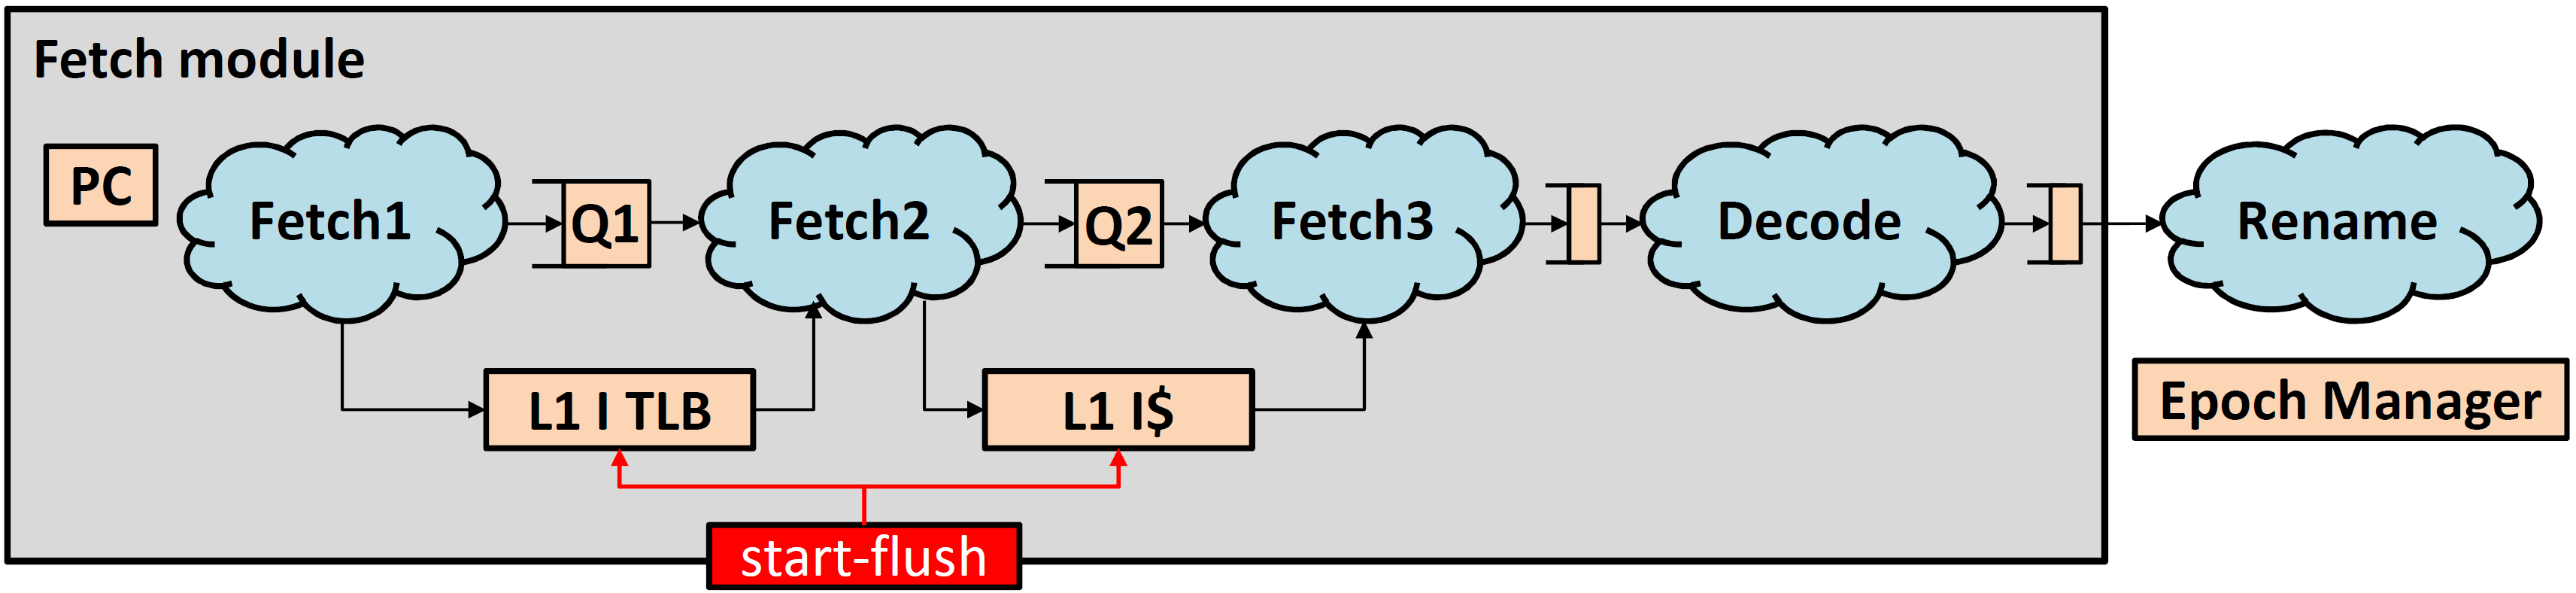
\includegraphics[width=\columnwidth]{fetch.PNG}
    \caption{The Fetch module in RiscyOO. Branch predictors, including the branch target buffer, tournament direction predictor and return address stack, are not shown.}\label{fig:fetch}
\end{figure}

\section{Conclusion}\label{sec:conclude}
To fully benefit from the openness of RISC-V, the architecture community needs a framework where many different people can cooperate to try out new ideas in real hardware.
Although existing chip generators can connect parameterized building blocks together,  they do not allow frequent changes to the building blocks.
We have also shown that latency-insensitive interfaces alone are insufficient in processor designs.
In this paper, we have proposed the CMD framework in which modules have guarded interface methods, and are composed together using atomic actions. 
With the atomicity guarantee in CMD, modules can be refined selectively relying only on the interface details, including Conflict Matrix, of other modules.
We have shown the efficacy of CMD by designing an OOO processor which has fairly complex architectural features.
Both the synthesis results and the performance results are very encouraging, and with sufficient effort by the community, it should be possible to deliver commercial grade OOO processors in not too distant a future.

\section*{Acknowledgment}
We thank all the anonymous reviewers for their helpful feedbacks on improving this paper.
We also benefited from the help from Jamey Hicks and Muralidaran Vijayaraghavan.
We thank Bluespec, Inc. for providing free tool licenses.
This research is supported by the Defense Advanced Research Projects Agency (DARPA) under Contract No. FA8750-16-2-0004 and Contract No. HR001118C0018.
Any opinions, findings and conclusions or recommendations expressed in this material are those of the authors and do not necessarily reflect the views of DARPA.

\begin{thebibliography}{10}
    \providecommand{\url}[1]{#1}
    \csname url@samestyle\endcsname
    \providecommand{\newblock}{\relax}
    \providecommand{\bibinfo}[2]{#2}
    \providecommand{\BIBentrySTDinterwordspacing}{\spaceskip=0pt\relax}
    \providecommand{\BIBentryALTinterwordstretchfactor}{4}
    \providecommand{\BIBentryALTinterwordspacing}{\spaceskip=\fontdimen2\font plus
        \BIBentryALTinterwordstretchfactor\fontdimen3\font minus
        \fontdimen4\font\relax}
    \providecommand{\BIBforeignlanguage}[2]{{%
            \expandafter\ifx\csname l@#1\endcsname\relax
            \typeout{** WARNING: IEEEtran.bst: No hyphenation pattern has been}%
            \typeout{** loaded for the language `#1'. Using the pattern for}%
            \typeout{** the default language instead.}%
            \else
            \language=\csname l@#1\endcsname
            \fi
            #2}}
    \providecommand{\BIBdecl}{\relax}
    \BIBdecl
    
    % reference 1
    \bibitem{rocketchip}
    ``Rocket chip generator,''
    \url{https://github.com/freechipsproject/rocket-chip}.
    
    % reference 2
    \bibitem{boom}
    ``Berkeley out-of-order machine,'' \url{https://github.com/ucb-bar/riscv-boom}.
    
    % reference 3
    \bibitem{fabscalar}
    N.~Choudhary, S.~Wadhavkar, T.~Shah, H.~Mayukh, J.~Gandhi, B.~Dwiel, S.~Navada,
    H.~Najaf-abadi, and E.~Rotenberg, ``Fabscalar: Automating superscalar core
    design,'' \emph{IEEE Micro}, vol.~32, 2012.
    
    % reference 4
    \bibitem{pulp}
    ``{PULP} platform,'' \url{https://github.com/pulp-platform}.
    
    % reference 5
    \bibitem{rosenband2005hardware}
    D.~L. Rosenband and Arvind, ``Hardware synthesis from guarded atomic actions
    with performance specifications,'' in \emph{ICCAD-2005. IEEE/ACM
        International Conference on Computer-Aided Design, 2005.}\hskip 1em plus
    0.5em minus 0.4em\relax IEEE, 2005.
    
    % reference 6
    \bibitem{riscv}
    ``Risc-v instruction set,'' \url{https://riscv.org/}.
    
    % reference 7
    \bibitem{awsf1}
    ``Amazon {EC2 F1} instances,''
    \url{https://aws.amazon.com/ec2/instance-types/f1/}.
    
    % reference 8
    \bibitem{riscyoo}
    S.~Zhang, A.~Wright, T.~Bourgeat, and Arvind, ``Composable building blocks to
    open up processor design,'' in \emph{2018 51st Annual IEEE/ACM International
        Symposium on Microarchitecture (MICRO)}.\hskip 1em plus 0.5em minus
    0.4em\relax IEEE, 2018.
    
    % reference 9
    \bibitem{translationCache}
    T.~W. Barr, A.~L. Cox, and S.~Rixner, ``Translation caching: skip, don't walk
    (the page table),'' \emph{ACM SIGARCH Computer Architecture News}, vol.~38,
    2010.
    
    % reference 10
    \bibitem{wmm}
    S.~Zhang, M.~Vijayaraghavan, and Arvind, ``Weak memory models: Balancing
    definitional simplicity and implementation flexibility,'' in \emph{Parallel
        Architectures and Compilation Techniques (PACT), 2017 26th International
        Conference on}.\hskip 1em plus 0.5em minus 0.4em\relax IEEE, 2017.
    
    % reference 11
    \bibitem{gam}
    S.~Zhang, M.~Vijayaraghavan, A.~Wright, M.~Alipour, and Arvind, ``Constructing
    a weak memory model,'' in \emph{Proceedings of the 45th Annual International
        Symposium on Computer Architecture}.\hskip 1em plus 0.5em minus 0.4em\relax
    IEEE Press, 2018.
    
\end{thebibliography}

\section*{Authors' Biography}

\begin{description}
    \item[Sizhuo Zhang] is a Ph.D. student at the Massachusetts Institute of Technology (MIT).
    His research interests include processor design, memory system, and accelerators.
    Zhang received an M.S. from MIT.
    He is a student member of the IEEE and ACM.
    Contact him at szzhang@csail.mit.edu.
    
    \item[Andrew Wright] is a Ph.D. student at the Massachusetts Institute of Technology (MIT).
    His research interests include flexible processor design, accelerators, and processor specification and verification.
    Wright received an S.M. in electrical engineering and computer science from MIT.
    He is a student member of the IEEE.
    Contact him at acwright@mit.edu.
    
    \item[Thomas Bourgeat] is a Ph.D. student at the Massachusetts Institute of Technology (MIT).
    His research interests include processor design, programming languages and formal methods.
    Bourgeat received an M.S. from University Paris Diderot.
    He is a student member of the ACM.
    Contact him at bthom@csail.mit.edu.
    
    \item[Arvind] is the Johnson Professor of Computer Science and Engineering at the Massachusetts Institute of Technology, where he is a member of the Computer Science and Artificial Intelligence Laboratory.
    His research interests include parallel systems and software, highlevel hardware synthesis languages, and enabling rapid development of embedded systems.
    Arvind received a Ph.D. in computer science from the University of Minnesota, Minneapolis.
    He is a Fellow of the IEEE and the ACM and a member of the National Academy of Engineering.
    Contact him at arvind@csail.mit.edu.
\end{description}

\end{document}
